\section{Models and Hierarchy}
In this chapter we are going to talk about the models and their hierarchy. As the architecture states, every model has to notify changes to his mediator that propagates on his object3D the modifications. The work needs those main models:
\begin{itemize}
\item Environment
\item Ground
\item Turret with the bullets
\item Storm which contains a number of enemies
\end{itemize}
A good source where to get the models and the textures is the website \textit{clara.io} where we got the Ground, the turret and the enemy in the \textit{collada} format, loading them with the colladaLoader.\\
So let see an overview of our chosen organization of the project.
\begin{figure}[h!]
\begin{center}
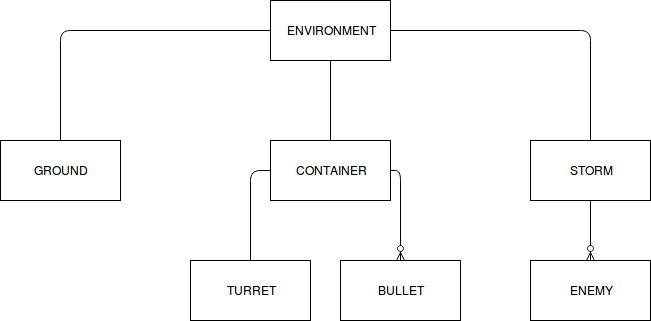
\includegraphics[scale=0.5]{images/models-diagram.jpg}
\caption{An ER style diagram of the objects hierarchy}
\end{center}
\end{figure}
The Environment is a big container, and the Ground is a standalone component, they are not interesting as the other two.
\newpage
\subsubsection{Turret/Bullet}
They are children of the same container because (as we'll see into the animation section) the bullet's animation starts from the turret's position but must not be influenced by its movement.\\
The turret is probably the most complex model into the project. The model downloaded from \textit{clara.io} was a single block, so we needed to separate it into three parts:
\begin{figure}[h!]
\begin{center}
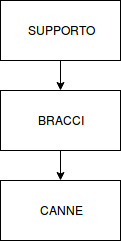
\includegraphics[scale=0.5]{images/turret-diagram.jpg}
\caption{A simple representation of the turret parts in a diagram.}
\end{center}
\end{figure}\\
Subdivision of the turret's parts required the use of the Blender 3D modeling software in order to obtain the parts previously described in the  tridimensional model used in the project. In the following image you can see the result obtained by the hierarchical subdivision of the model in the application:
\begin{figure}[h!]
\begin{center}
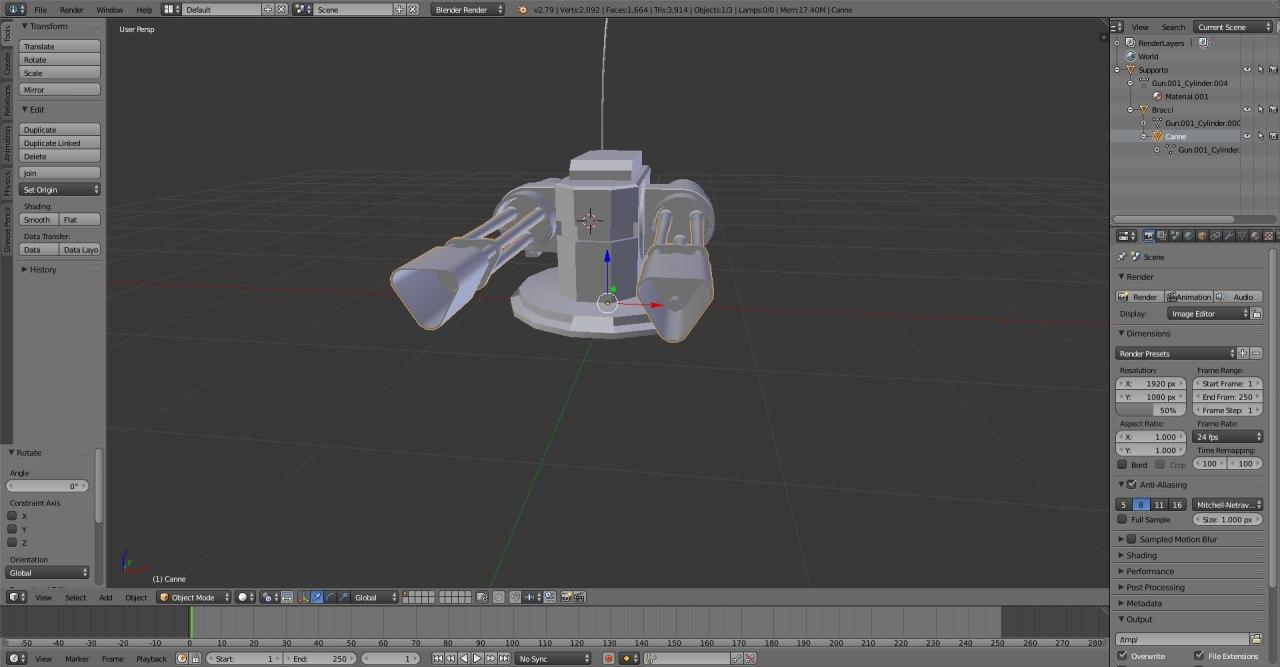
\includegraphics[scale=0.35]{images/turret-blender.jpg}
\caption{Turret 3D model hierarchical subdivision in Blender.}
\end{center}
\end{figure}
There is not so much to say about the bullet, it is a very simple sphere, with a yellow basic Mesh Material. It's object3D is encapsulated into the BulletMediator that is child of the TurretMediator.
\subsubsection{Storm}
The \textit{Storm} is the enemies' container into the classic mode, it's just a transparent inclined plane containing all the enemies, it allows us to control all the enemies movements simply using the \textit{x} and \textit{y} axes without worrying about the \textit{z} one. As a final result a clear descending movement directed towards the player is obtained, correcting also the enemy invaders' inclinations.
\begin{figure}[h!]
\begin{center}
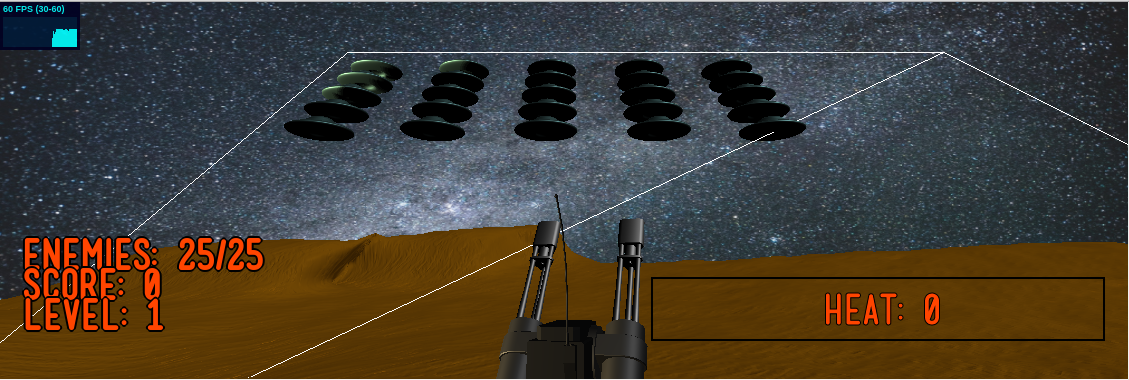
\includegraphics[scale=0.3]{images/storm-plane.png}
\caption{How the plane would appear}
\end{center}
\end{figure}
\newpage
\subsubsection{TPStorm}
The \textit{TPStorm (TwoPointStorm)} is an extension of the previously described Storm where the movements of the enemies are handled in a more freely way. \\
The number of enemies loaded in scene depends on how many enemies will be displayed on the screen during wave, and is defined and can be adjusted in the model by acting on one of its parameters. When the storm is build up, enemies are positioned in equal number on two different spawning points that are located over the camera's visible way. \\
During a wave, at temporized intervals an enemy is selected and starts to move from its spawning point entering in the player's visible area, making displacements under a set of random positions of fixed length, defined under boundaries that involve all the axes. In other terms the random positions are selected in a parallelepiped enclosed in the player's field of vision. \\
After all random positions have been reached, the enemy is guided to reach a final position randomly chosen among six predefined available.
\begin{figure}[h!]
\begin{center}
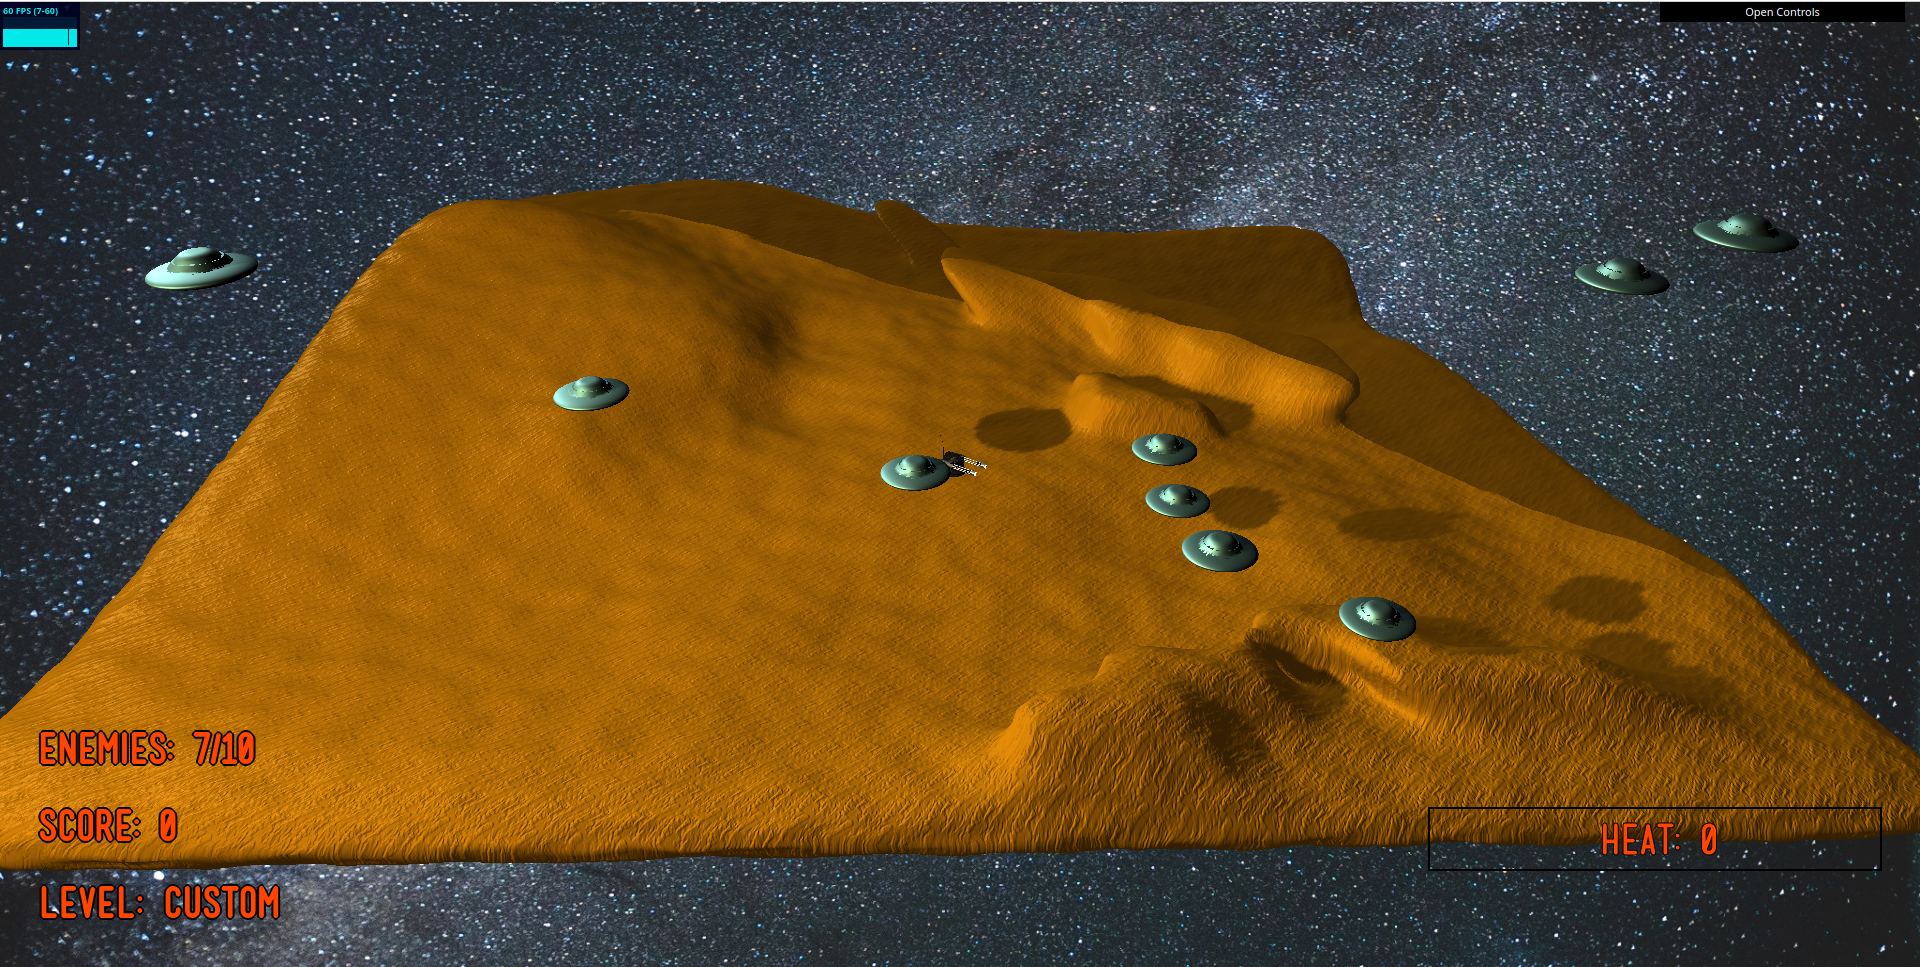
\includegraphics[scale=0.22]{images/tps-orbitview.png}
\caption{\textit{TPStorm} appearance obtained by moving the camera.}
\end{center}
\end{figure}